\documentclass[tikz,border=10pt]{standalone}
\usetikzlibrary{patterns}
\usepackage{amsmath, amssymb}

\begin{document}
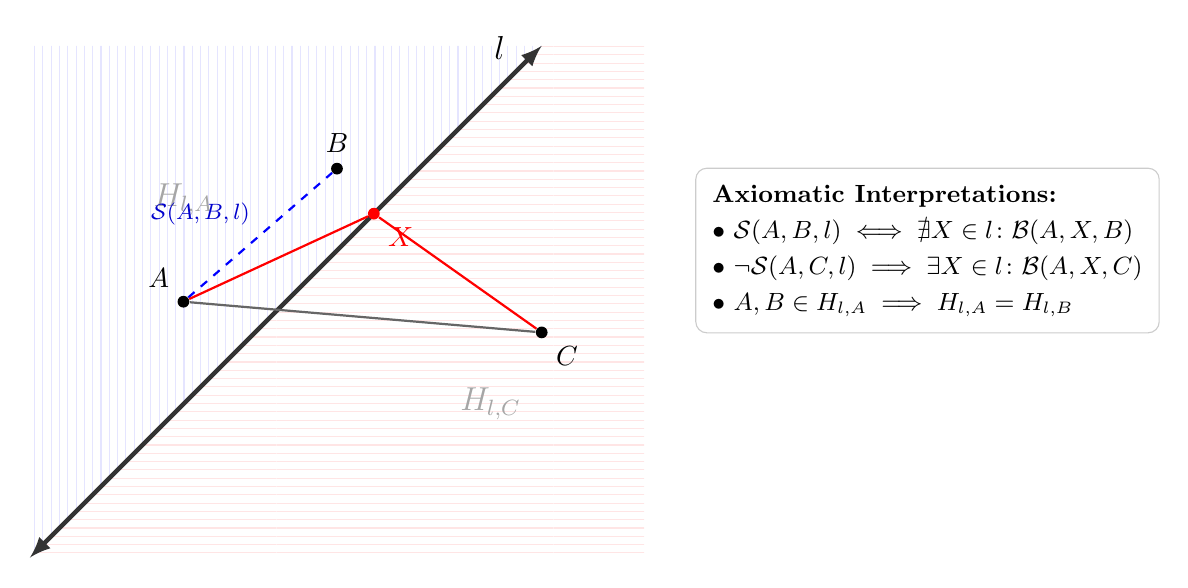
\begin{tikzpicture}[>=stealth, scale=1.3]

  % Styles
  \tikzset{
    point/.style={circle, fill=black, inner sep=1.5pt},
    line label/.style={font=\small, fill=white, inner sep=2pt},
    region label/.style={font=\large\bfseries, color=gray!70}
  }

  % --- BACKGROUND PATTERNS FOR HALF-PLANES ---
  % Left/Top Half-Plane (H_{l,A}) - Soft vertical lines
  \path[pattern=vertical lines, pattern color=blue!10] (-3.5, -2) -- (1.5, 3) -- (-3.5, 3) -- cycle;
  % Right/Bottom Half-Plane (H_{l,C}) - Soft horizontal lines
  \path[pattern=horizontal lines, pattern color=red!10] (-3.5, -2) -- (1.5, 3) -- (2.5, 3) -- (2.5, -2) -- cycle;

  % --- THE PARTITIONING LINE ---
  % Line l: y = x + 1.5 roughly
  \draw[latex-latex, ultra thick, draw=black!80] (-3.5, -2) -- (1.5, 3)
    node[pos=0.95, above left, font=\large] {$l$};

  % --- REGION LABELS (Equivalence Classes / Half-Planes) ---
  \node[region label] at (-2, 1.5) {$H_{l,A}$};
  \node[region label] at (1, -0.5) {$H_{l,C}$};

  % --- POINTS ---
  % Same side elements (A and B)
  \node[point, label=above left:$A$] (A) at (-2, 0.5) {};
  \node[point, label=above:$B$] (B) at (-0.5, 1.8) {};

  % Opposite side element (C)
  \node[point, label=below right:$C$] (C) at (1.5, 0.2) {};

  % Intersection point on line l
  \node[point, fill=red, label=below right:\color{red}$X$] (X) at (-0.14, 1.36) {};

  % --- CONNECTIONS & RELATIONS ---
  % Same-Side Path (No intersection with l)
  \draw[thick, blue, dashed] (A) -- (B)
    node[midway, above left, font=\footnotesize, text=blue!80!black] {$\mathcal{S}(A,B,l)$};

  % Opposite-Side Path (Intersects l at X)
  \draw[thick, black!60] (A) -- (C);

  % Highlight the segment portion indicating betweenness
  \draw[thick, red] (A) -- (X) -- (C);

  % --- ANNOTATION KEY ---
  \node[right, font=\small, align=left, fill=white, draw=gray!40, rounded corners, inner sep=6pt] at (3, 1) {
    \textbf{Axiomatic Interpretations:}\\[2pt]
    $\bullet\ \mathcal{S}(A,B,l) \iff \nexists X \in l \colon \mathcal{B}(A,X,B)$ \\[2pt]
    $\bullet\ \neg\mathcal{S}(A,C,l) \implies \exists X \in l \colon \mathcal{B}(A,X,C)$ \\[2pt]
    $\bullet\ A, B \in H_{l,A} \implies H_{l,A} = H_{l,B}$
  };

\end{tikzpicture}
\end{document}
